\documentclass{article}
\usepackage[UTF8]{ctex}
\usepackage{geometry}
\usepackage{natbib}
\geometry{left=3.18cm,right=3.18cm,top=2.54cm,bottom=2.54cm}
\usepackage{graphicx}
\pagestyle{plain}	
\usepackage{setspace}
\usepackage{caption2}
\usepackage{datetime} %日期
\usepackage{float}
\renewcommand{\today}{\number\year 年 \number\month 月 \number\day 日}
\renewcommand{\captionlabelfont}{\small}
\renewcommand{\captionfont}{\small}
\begin{document}

\begin{figure}
    \centering
    
\includegraphics[width=8cm]{upc.png}

    \label{figupc}
\end{figure}

	\begin{center}
		\quad \\
		\quad \\
		\heiti \fontsize{45}{17} \quad \quad \quad 
		\vskip 1.5cm
		\heiti \zihao{2} 《计算科学导论》课程总结报告
	\end{center}
	\vskip 2.0cm
		
	\begin{quotation}
% 	\begin{center}
		\doublespacing
		
        \zihao{4}\par\setlength\parindent{7em}
		\quad 

		学生姓名:\underline{\qquad  万舒成 \qquad \qquad}

		学\hspace{0.61cm} 号:\underline{\qquad 2007010221\qquad}
		
		专业班级:\underline{\qquad 本研一体化(人工智能) 2001\qquad  }
		
        学\hspace{0.61cm} 院:\underline{计算机科学与技术学院}
% 	\end{center}
		\vskip 2cm
		\centering
		\begin{table}[h]
            \centering 
            \zihao{4}
            \begin{tabular}{|c|c|c|c|c|c|c|}
            % 这里的rl 与表格对应可以看到,姓名是r,右对齐的;学号是l,左对齐的;若想居中,使用c关键字。
                \hline
                课程认识 & 问题思 考 & 格式规范  & IT工具  & Latex附加  & 总分 & 评阅教师 \\
                30\% & 30\% & 20\% & 20\% & 10\% &  &  \\
                \hline
                 & & & & & &\\
                & & & & & &\\
                \hline
            \end{tabular}
        \end{table}
		\vskip 2cm
		\today
	\end{quotation}

\thispagestyle{empty}
\newpage
\setcounter{page}{1}
% 在这之前是封面,在这之后是正文
\section{引言}
《计算科学导论》(赵致琢著)第3版分为五章内容,分别为引论;计算科学的基本概念和基本知识;计算科学:它的意义、内容和方法;如何学习计算科学和健康成长;布尔代数基础。每章内容都分出很多内容,每个内容都包括一个方面的知识,比较全面。本次课程总结报告采取引言,对计算科学导论这门课程的认识、体会,进一步的思考,总结,参考文献,附录的大纲来展现。

\section{对计算科学导论这门课程的认识、体会}
计算科学导论一共32个学时,是一门学科入门性导引课程。对于一个刚刚接触计算机的萌新来说,尽管导论已经尽量将里面的内容大众化,但是仍然会有些听不懂,对于一些专有名词也是不能理解。通过计算科学导论,我们可以了解到一些计算学科的基本知识和学科方法论,比如计算模型,二进制,机器语言与汇编语言,算法,科学哲学,科学方法论等。同时了解计算领域的热点,如深度学习,人机交互,机器学习等。作为一个导引性的教材,《计算科学导论》以科普的形式为初入计算机学科者提供一个了解和学习计算机科学与技术的导引,我们不能从导论中学到大量计算机科学与技术领域的专门的、具体的、系统的专业技术知识。因为虽然导论涉及的内容很广,但是对知识的解读都比较浅,不太深,所以我们并不能通过导论搞透一个知识点。例如第二章第九节的逻辑与人工智能,在书中只介绍了人工智能产生的源头,将逻辑与计算机结合在一起而成的人工智能,并没有对其进行详细的解释,我们只能知道大概的意思但要细究还是不清楚。还有就是第二章第十三节的高性能计算,书中只讲了高性能计算的概念、分类、发展、特性和意义,对其中涉及的具体技术也没有详细的展开,只让我们对这个名词有一定的印象,但是并不完全懂。


\section{进一步的思考}
由我和代鹏同学合作完成的分组演讲讲述了云盘的相关内容,其中涉及到了云盘的定义、功能、发展历程和发展前景。

\begin{itemize}
    \item 云盘是云储存的一种,其中用到了计算机的云储存技术。\par
    云存储系统对外提供多种不同的存储服务,各种服务的数据统一存放在云存储系统中,形成一个海量数据池。云存储的数据存储层将不同类型的存储设备互连起来,实现海量数据的统一管理,同时实现对存储设备
    的集中管理、状态监控以及容量的动态扩展,实质是一种面向服务的分布式存储系统。\cite{yunchucun} \par
    云盘公司先创立一个云储存系统,然后通过云盘构建用户与系统之间的联系,用户通过云盘访问云储存系统,进行内容的存储和提取。现在的云储存系统有一种功能:有一个用户上传了一个内容,当另一个用户上传相同的内容时,系统不再拿出一个位置来储存,而是单单把这个内容的使用权改为这两个用户,这样既能减少系统的维护成本,也能更有效地使用数据。目前随着用户使用的空间越来越大,U盘固定内存大小的弊端就显现出来了,网盘免费使用的内存大小就已经够大部分人日常使用,但是一些企业和老师等信息量比较大的群体就需要更大的储存空间,频繁地更换U盘显然是不太合适的,一个很大的U盘价格也有点贵,相比之下,一个月10元2T内存的云盘就显得廉价很多。除此之外,安全,方便,稳定都是云盘相比U盘的优点。但是,使用云盘时仍然需要一个客户端,然后从中下载数据到本地电脑,这样就产生了一个新的问题:如果没有网络该怎么办,不能下载客户端,就算有客户端没有网络也不能访问到云储存系统,自然也不能下载自己网盘中的内容,这点在一些情况下就很致命,没办法解决,只能通过U盘解决或者通过局域网共享文件夹来解决。虽然现在百度网盘推出了网页版,但是仍然需要网络去完成操作。
    \item 云盘功能有搜索资源、储存下载、同步资源、自动备份、资源分享、在线播放等。\par
    对于同步资源的功能,云盘公司推出了一种叫做同步盘的东西,用户在使用时只需要登录并且创建一个同步文件夹就可以,用户将文件上传至同步文件夹,之后自己修改文件之后不需要再次上传文件,由同步盘自动实现文件同步,即实时更新文件状态,保证储存的文件都是最新版本。\par
    需要注意的是,同步盘与Pc客户端是有区别的。同步盘主
    要解决文件双向同步问题,本地同步文件夹数据同步到云端;
    云端数据增加、删除后本地也会随之变化,适合需要在多设备
    共享数据的办公人群使用。而Pc客户端主要是解决用户单向上
    传或下载文件的需求,用户可以根据自己的意愿上传、下载文
    件。同步功能非常实用,尤其是对于依赖电脑、手机来办公的
    工作者。\cite{gongneng}	 \par
    对于资源共享的功能,用户可以将自己云盘中的内容选择加密或者不加密的方式将这个内容分享给他人,如果加密的话就需要提取码,而这个提取码是随机产生的,由用户将提取码给他人,然后别人再用提取码去提取文件。这种方式可以很好的将资源分享给一部分人,但不给所有人下载使用,而这部分人数量还不少,如果一个一个发的话太麻烦了,加密分享并且提供提取码就是很好的解决方法。在干货博主,教师和公司人员等这些职业的人员来说,这项功能就很实用,能够将资源局限在自己想要分享的圈子中。例如,干货博主只想将资源分享给自己的粉丝或者关注自己的人、教师只想将学习资源分享给自己的学生、公司人员只想将工作资源分享给自己的同事,如果将资源外传就可能会加大竞争压力。用户除了自己主动分享内容,还可以在云盘中创建一个共享文件夹,多个用户可以共同上传和下载共享文件夹中的内容,这种形式相比前面的更加实用一些,不过这种形式可能因为后期文件太多而寻找有困难。 \par
    其他功能就比较常规了,但是在线播放功能确实为用户查看文件提供了很大的便捷,不需要说看一个文件无论大小都需要下载才能观看,减少用户操作步骤,提升用户体验。
    \item 云盘的发展历程可谓是困难重重。在云盘刚刚兴起的时期,网络上仍然存在很多的盗版网址,各种资源都可以从盗版网址中获取,云盘的使用量很少,存在感很低。后来随着网络的整治,各大盗版网站相继被封,云盘的用途逐渐显现出来。云盘作为一项软件型技术,发展历程主要还是各大云盘软件之间的竞争。刚开始为了吸引用户都会采取送福利的方式,只有保障自己的用户基础,才能谈以后的盈利空间。但是又因为云盘的免费福利过多,基本满足个人的需求,所以愿意为云盘买单的用户少之又少,只有少数需要大量储存空间的人群才需要充值购买VIP。因为云盘的盈利模式不理想,所以在这之后各大云盘厂商就开始剥削原有用户的权力,消减空间,限制上传下载的速度,限制上传大小,甚至还有的云盘公司为了牟利,利用云盘大量向用户投放广告,导致用户一步步反感,纷纷开始使用其他方式储存资源,比如利用贴吧论坛等渠道发布资源,然后需要时再下载。虽然可以通过论坛等平台发布资源,但是有一些特别的资源只能通过网盘储存并且分享。在2016年打击利用云盘传播淫秽色情信息专项整治行动的全面展开,很多平台因此纷纷选择关闭部分功能或者直接停止个人服务。比如当时的巨头360云盘因为用户往云盘中存放大量色情信息,进行非法交易等行为,最后只好让用户在半年时间内转移所有的资源,但网速仅为1kb/s,半年后关闭了360云盘功能。2017年,行业洗牌逐渐完成,个人云盘市场回归理性,商业模式形成,在AI技术赋能下走向个性化服务。
    
    \item 后来云盘逐渐分为两类:个人云盘和企业云盘。
    自2016年"净网行动"以来,个人云盘服务商对用户存储内容的主动监管就成为一项不可避免的成本。数以亿计的用户在个人云盘中存储了海量的数据,服务商如果审核不到位、不即使,就意味着其将随时面临品牌商誉受损甚至是关停服务的风险。现阶段AI技术已经在内容审核工作中得到广泛应用。基于深度识别算法构建的模型,能够对复杂数据进行有效解读,以辅助传统的人工审核。对于个人云盘行业而言,AI在后台审查中将充分发挥降本增效的优势,大幅减少盗版侵权和淫秽色情信息在用户间的分享和传播。在前台面向用户的层面,利用AI技术的个人云盘将可以采用更加智能化的方式帮助用户提高数据管理的效率,进一步优化用户使用体验。由于智能手机满足了人们的日常拍摄需求,大量的照片备份需要备份到云端。通过对拍摄的时间、地点以及对象进行多维度的智能分类,个人云盘将为用户的图片管理和搜索提供极大的便利。\cite{gerenyunpan}
在2014年的好莱坞艳照门事件中,就是由于云盘的漏洞,让黑客钻了空子,最终造成严重的后果。我们不禁会怀疑云盘的安全性,储存在云盘中的内容是否会被他人利用或者盗取。云盘公司也开始使用新技术去填补漏洞,保障用户的信息安全。In IV phase, the data owner interacts with the n cloud servers through challenge‐response protocol to check the correctness of outsourced data. This is performed by randomly checking a subset of segments from each coded block in the server. The IV phase mainly consists of three steps: challenge, proof generation, and proof verification. The data owner sends the audit queries in the challenge step, which consists of the index of the challenged segments and random coefficients to generate the linear combination. In proof generation step, each cloud server, say i, responds to the audit queries by generating a linear combination of challenged encrypted segments and authentication tags, corresponding to each coded block as shown in Figure 3. The data owner performs the integrity check in proof verification step by first decrypting the retrieved encrypted segment, which is followed by tag computation. If this computed tag matches with the retrieved tag for all coded blocks in a server, then the server passes the integrity check. Otherwise, SR is initiated due to detection of data corruption.\cite{anquan}
    通过多个服务器交互,来检查外包数据的正确性,确保服务器的安全性,下面为文献中介绍的图3。
    \begin{figure}[H]
    	\centering
    	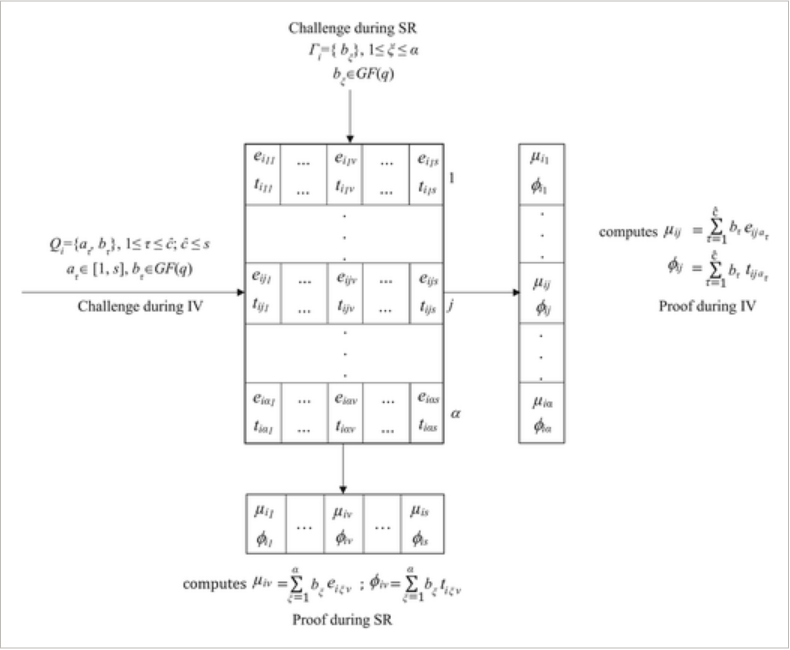
\includegraphics[width=0.7\linewidth]{图3}
    	\caption{}
    	\label{fig:3}
    \end{figure}
    
    个人云盘经过多年的发展,目前已经大致成形,发展空间很小,未来在这方面的创新几乎没有,只能不断地去完善它,所以,各大云盘商家纷纷开始向企业云盘发展,企图在企业云盘中抢占先机,率先占领市场。在企业中,工作人员的内存需求比较大,对云盘的要求比较高,可以通过企业云盘共同完成任务。相对于个人云盘,企业云盘的盈利空间更大,有比较固定的消费人群,自然,各大厂商向企业云盘这方面发展也是必然的。\par
    企业网盘是基于云计算理念推出的企业数据网络存储和管理解决方案,利用互联网后台数据中心的海量计算和存储能力为企业提供数据汇总分发、存储备份和管理等服务(该定义来自百度百科)。企业云盘将数据存放在私有云中又可以获得公有云计算资源,灵活性程度高,易扩展。在本次新冠肺炎疫情中,商业受到了重创,工厂不能够按时地开工,企业不能按时地回到岗位上班,导致许多公司破产倒闭,于是许多企业纷纷开始了“云办公”的模式,例如借用钉钉和Yotta企业云盘的平台,使得上班族坐在家中上班。因为大家不能集中在一起,但是信息又是需要共享的,企业云盘就很好地解决了这个问题,使得企业云盘在疫情期间大放光彩。企业云盘的安全性还是比较高的,到现在也没有出现什么影响比较大的报道说企业云盘信息泄露导致什么事情的发生,但我们仍要加强信息安全的建设,保证储存内容的绝对安全,因为这事关我们的隐私权和商业秘密。\par
    Finally, we implement the enterprise‐oriented private cloud storage system Frostor and deploy it on a 24‐node cluster in our data center. The evaluation with several experiments shows (1) our fine‐grained access control mechanism is able to prevent enterprise data from being accessed illegally and achieve internal data sharing and isolation, (2) our prefetching mechanism can predict future user accesses with an accuracy up to 80\%, and (3) our cache mechanism performs better than the other classical algorithms. By adopting the 2‐level performance optimization mechanism, Frostor can reduce at least 60\% of the access latency in many application scenarios. Our main contributions in this paper are A fine‐grained access control mechanism is proposed to solve the problem of secure data access in the enterprise cloud storage and to protect data privacy while sharing data inside the enterprise. A 2‐level performance optimization mechanism is adopted the improve the access performance of the enterprise cloud storage.A practical private cloud storage system Frostor is implemented based on GlusterFS. \cite{qiye}
    作者一行人研制出了一个专门的云储存系统Frostor,利用细粒度访问控制机制有效的阻止了企业数据被非法地访问,防止企业数据外泄,保护公司机密,同时增设预测机制,缓存机制,性能优化机制等减少访问延迟。该系统既解决了云盘的安全问题,又提高了云盘的访问性能,提升用户实际体验,可谓是企业云盘的一大突破。\par
    
\end{itemize}


\section{总结}
计算科学是对描述和变换信息的算法过程,包括其理论、分析、设计、效率、分析、实现和应用的系统的研究。计算机科学,研究计算机及其周围各种现象和规律的科学,亦即研究计算机系统结构、程序系统(即软件)、人工智能以及计算本身的性质和问题的学科。计算机科学是一门包含各种各样与计算和信息处理相关主题的系统学科,从抽象的算法分析、形式化语法等等,到更具体的主题如编程语言、程序设计、软件和硬件等。计算科学为人类认知世界提供了一种可能的有前途的方法,可能会引起人类世界观自然观的巨大变革。计算机科学和信息科学的极大成就促进了计算概念的普遍化。计算主义强纲领认为物理世界是可计算的,算法决定物理过程。进而,认知可计算主义为意识提供了一种主流的解释方法,为人工智能技术的发展提供了理论支撑。生命过程可计算主义为理解生命以及基因技术的发展和基于生命科学的计算机技术等提供了理论纲领。
计算机科学导论作为一门入门型导引课程,其扮演的作用就是在我们上一些专业课之前,先给我们讲授计算机学科的框架,了解一些专业知识的基本内容,目的也就是带我们进入计算机的世界,确定以后在计算机领域的发展方向,同时,让我们在接触相关知识时先有个大概的了解,学习起来就不会那么地吃力。本次报告,我思考了计算科学导论在学习方面的作用,同时根据书中讲授的内容思考了自己想要走的方向,为自己后面的个人职业规划提供一定的参考。同时,在上课的时候,老师也不单单只是讲课本上的内容,还会对其进行拓展,讲一些具体的例子,上课生动有趣,自然在所讲的内容方面也会提起兴趣,计算机课程本来就是比较抽象枯燥的,若提前一步提起兴趣,对以后的学习肯定会有很大的帮助。然后就是对分组演讲内容的进一步思考。从云盘的定义、功能、发展历程和应用前景方面对所讲内容做出进一步的思考,借助百度百科,知乎和各种论文了解到云盘的相关内容,然后根据这些资料,结合自己的想法,写出上面的内容。之前的新生研讨课报告也是使用latex来写的,但是也是时间紧没有学习太多的语法,只学习了一些基本的语法,这次计算科学导论虽然说也没有使用太多新的语法,但是还是花时间在B站上面系统性的学习了latex语法,这在我们写报告中有用,在我们以后写论文没有模板时,就显得非常的有用了,所以现在学好latex语法,非常有必要。

\section{附录}
    \begin{figure}[H]
    	\centering
    	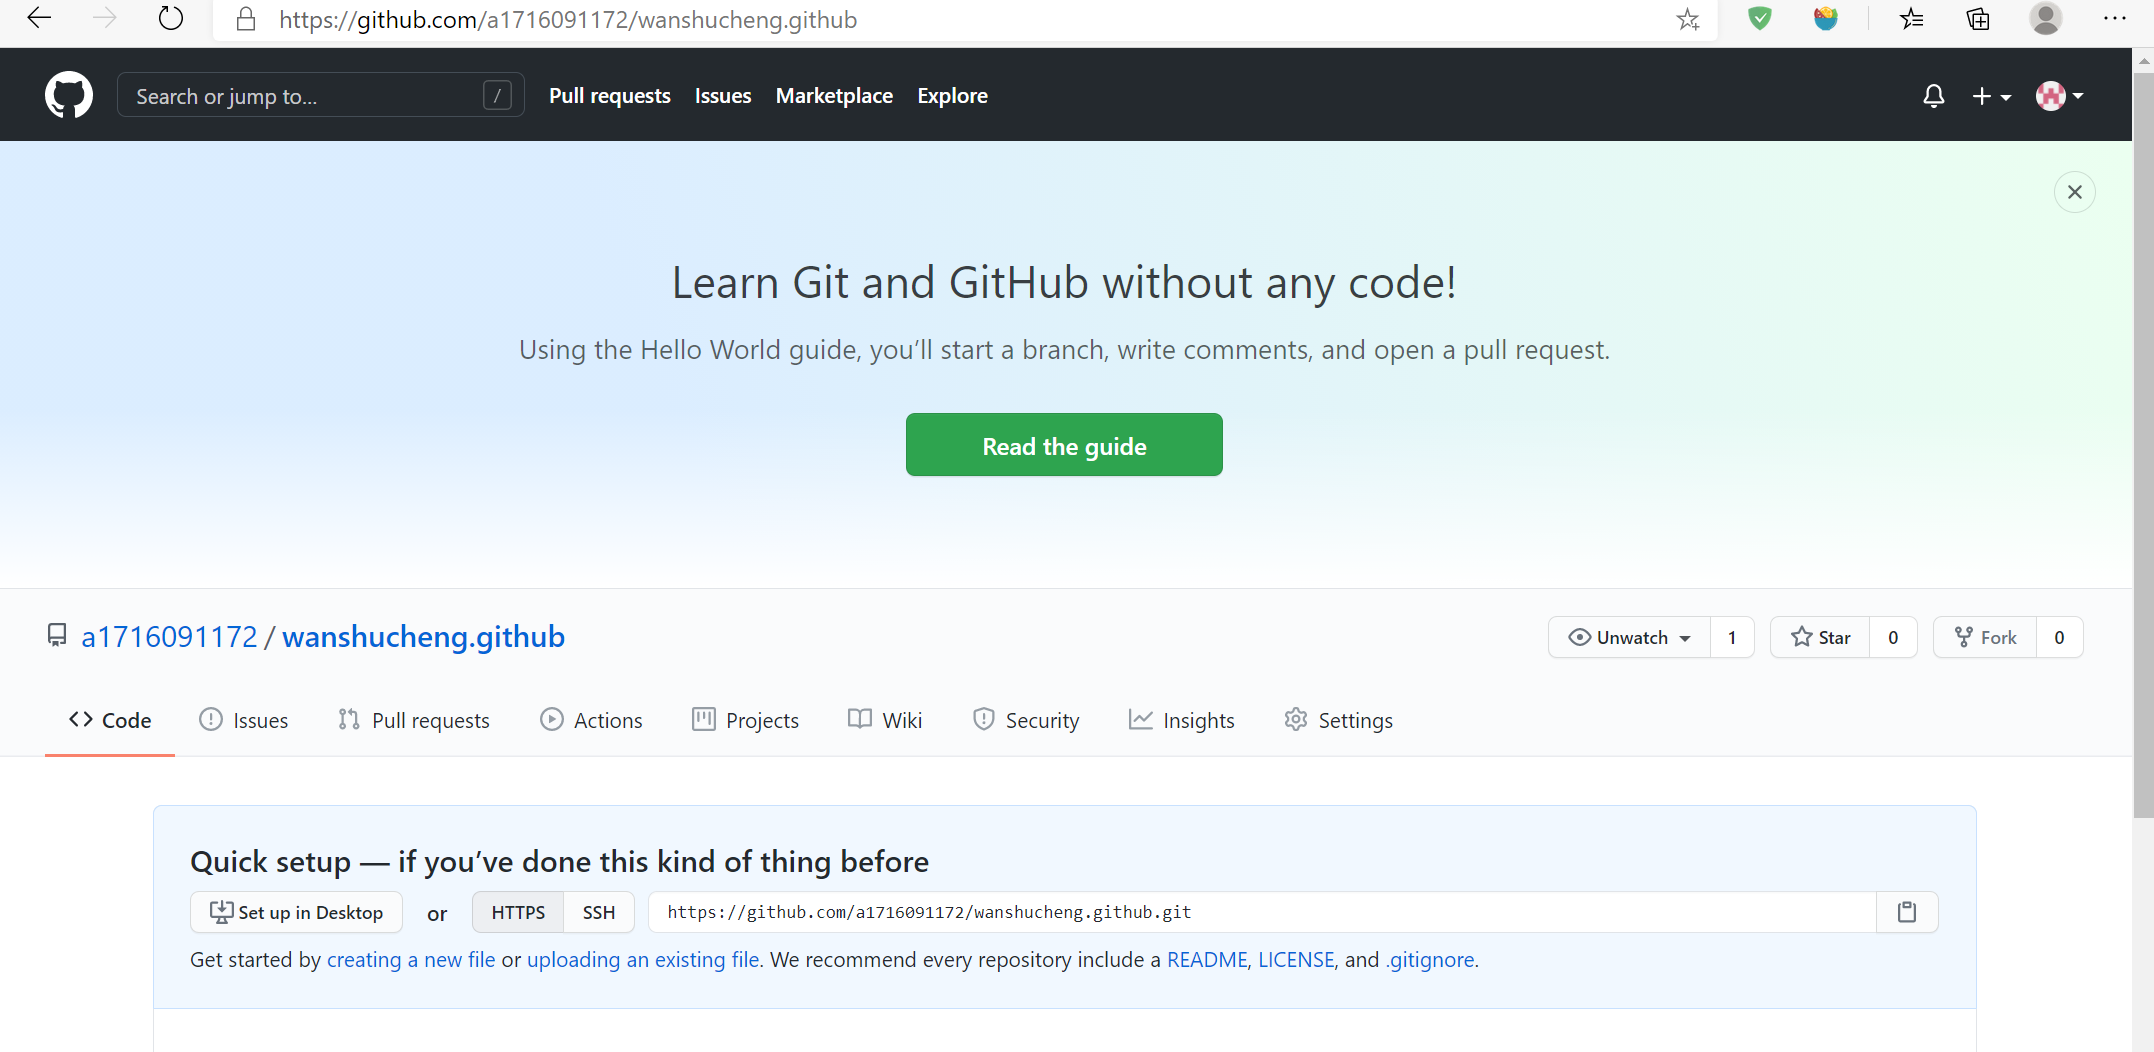
\includegraphics[width=0.7\linewidth]{Github}
    	\caption{}
    	\label{fig:github}
    	个人网址为:https://github.com/a1716091172/wanshucheng.github
    \end{figure}
	
    \begin{figure}[H]
    	\centering
    	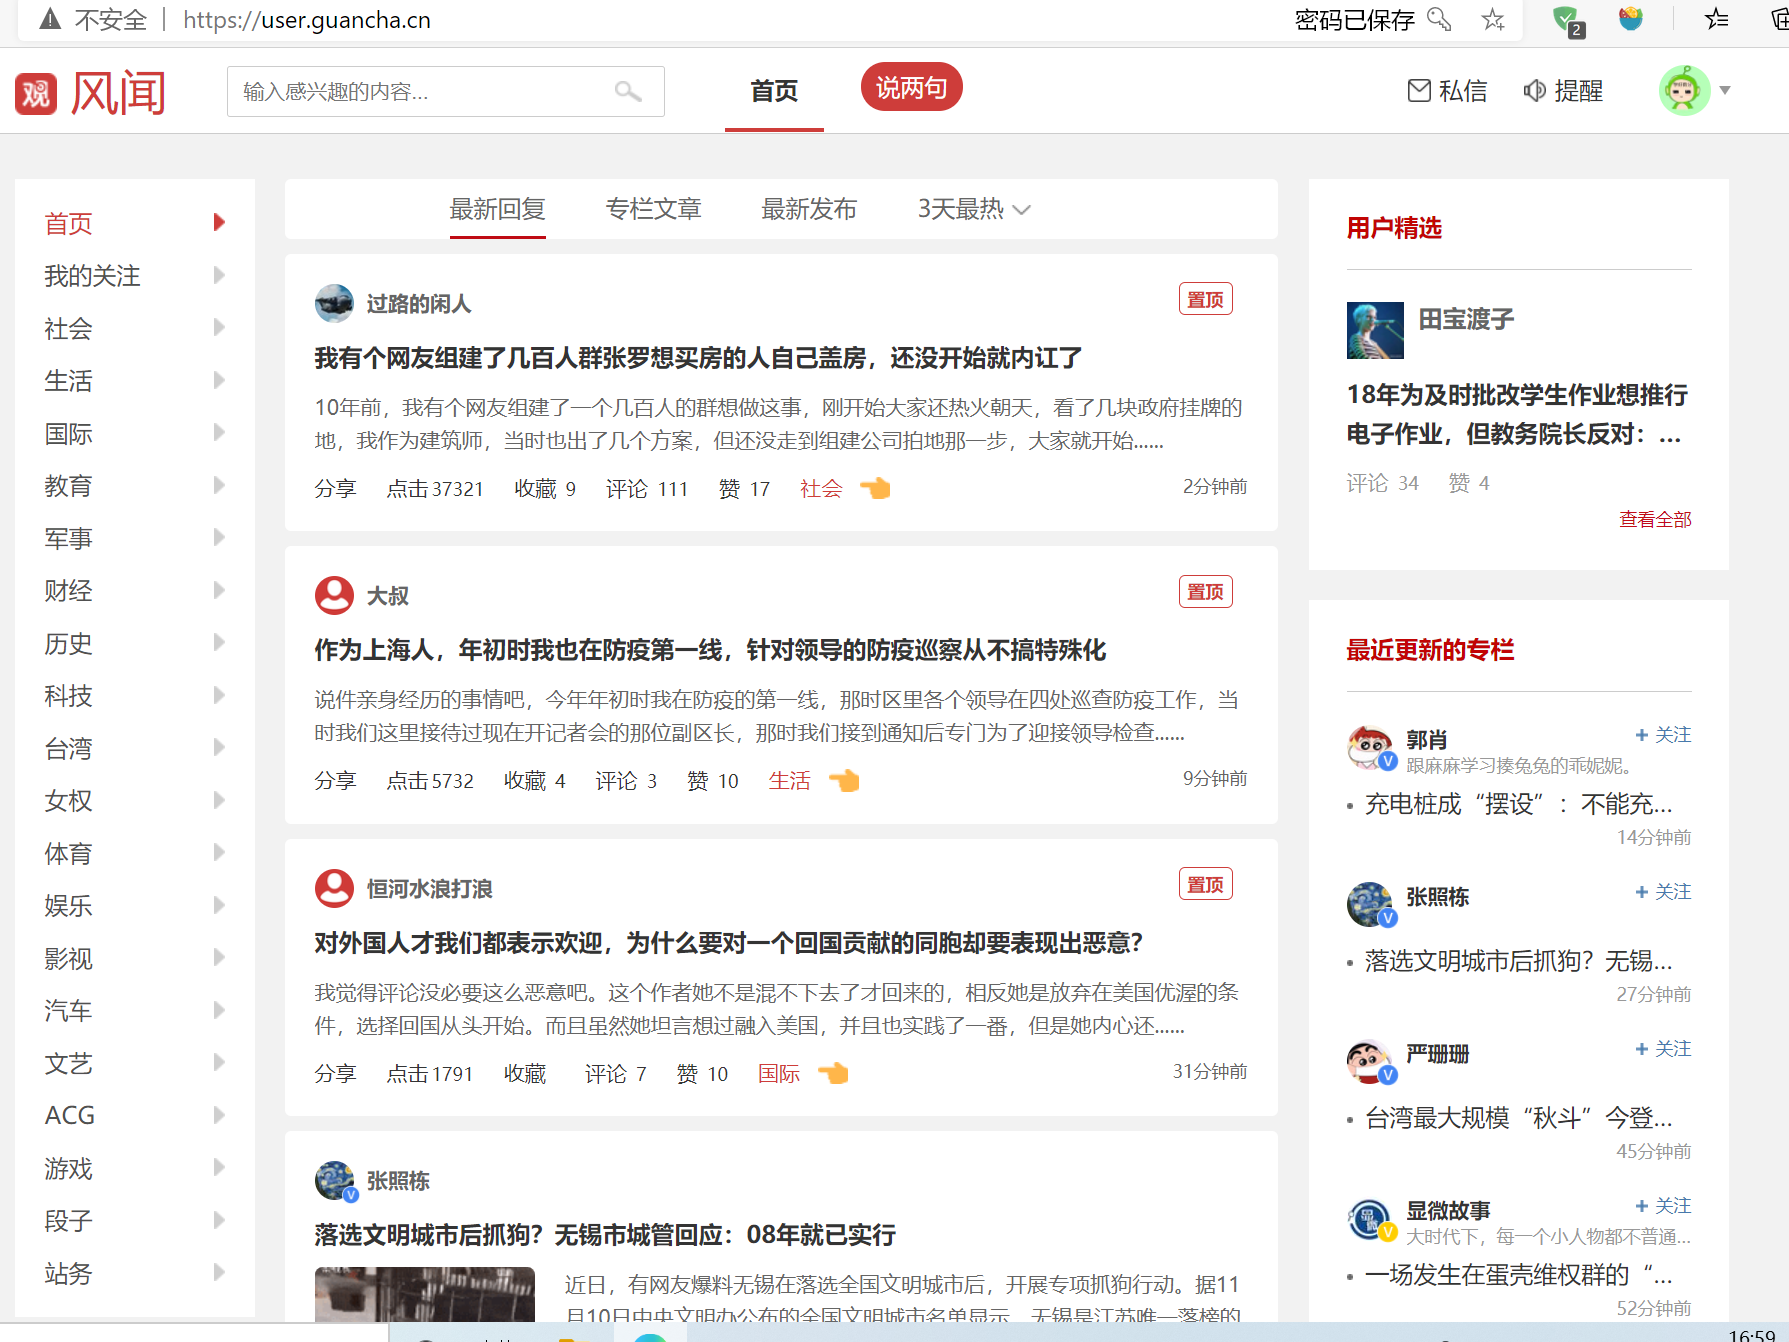
\includegraphics[width=0.7\linewidth]{观察者}
    	\caption{}
    	\label{fig:}
    \end{figure}
    
    \begin{figure}[H]
    	\centering
    	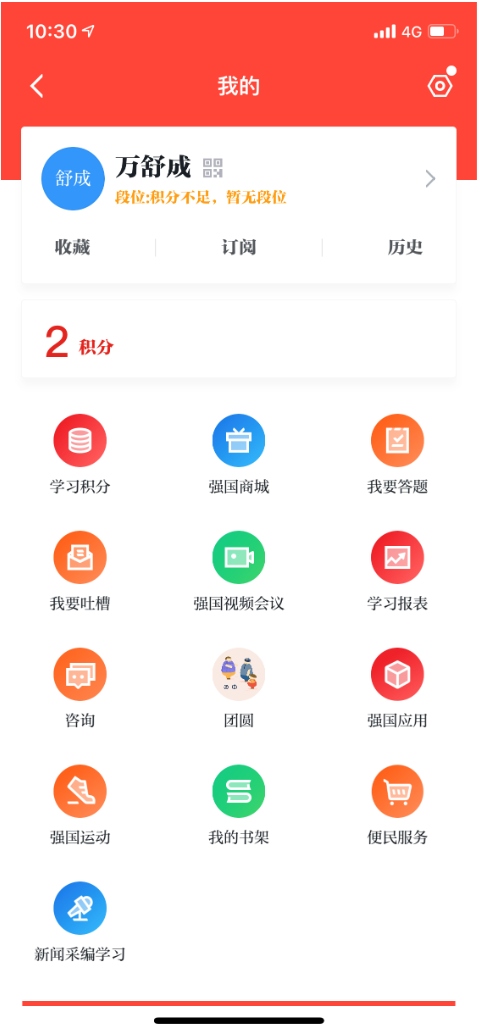
\includegraphics[width=0.7\linewidth]{学习强国}
    	\caption{}
    	\label{fig:}
    \end{figure}
    
    \begin{figure}[H]
    	\centering
    	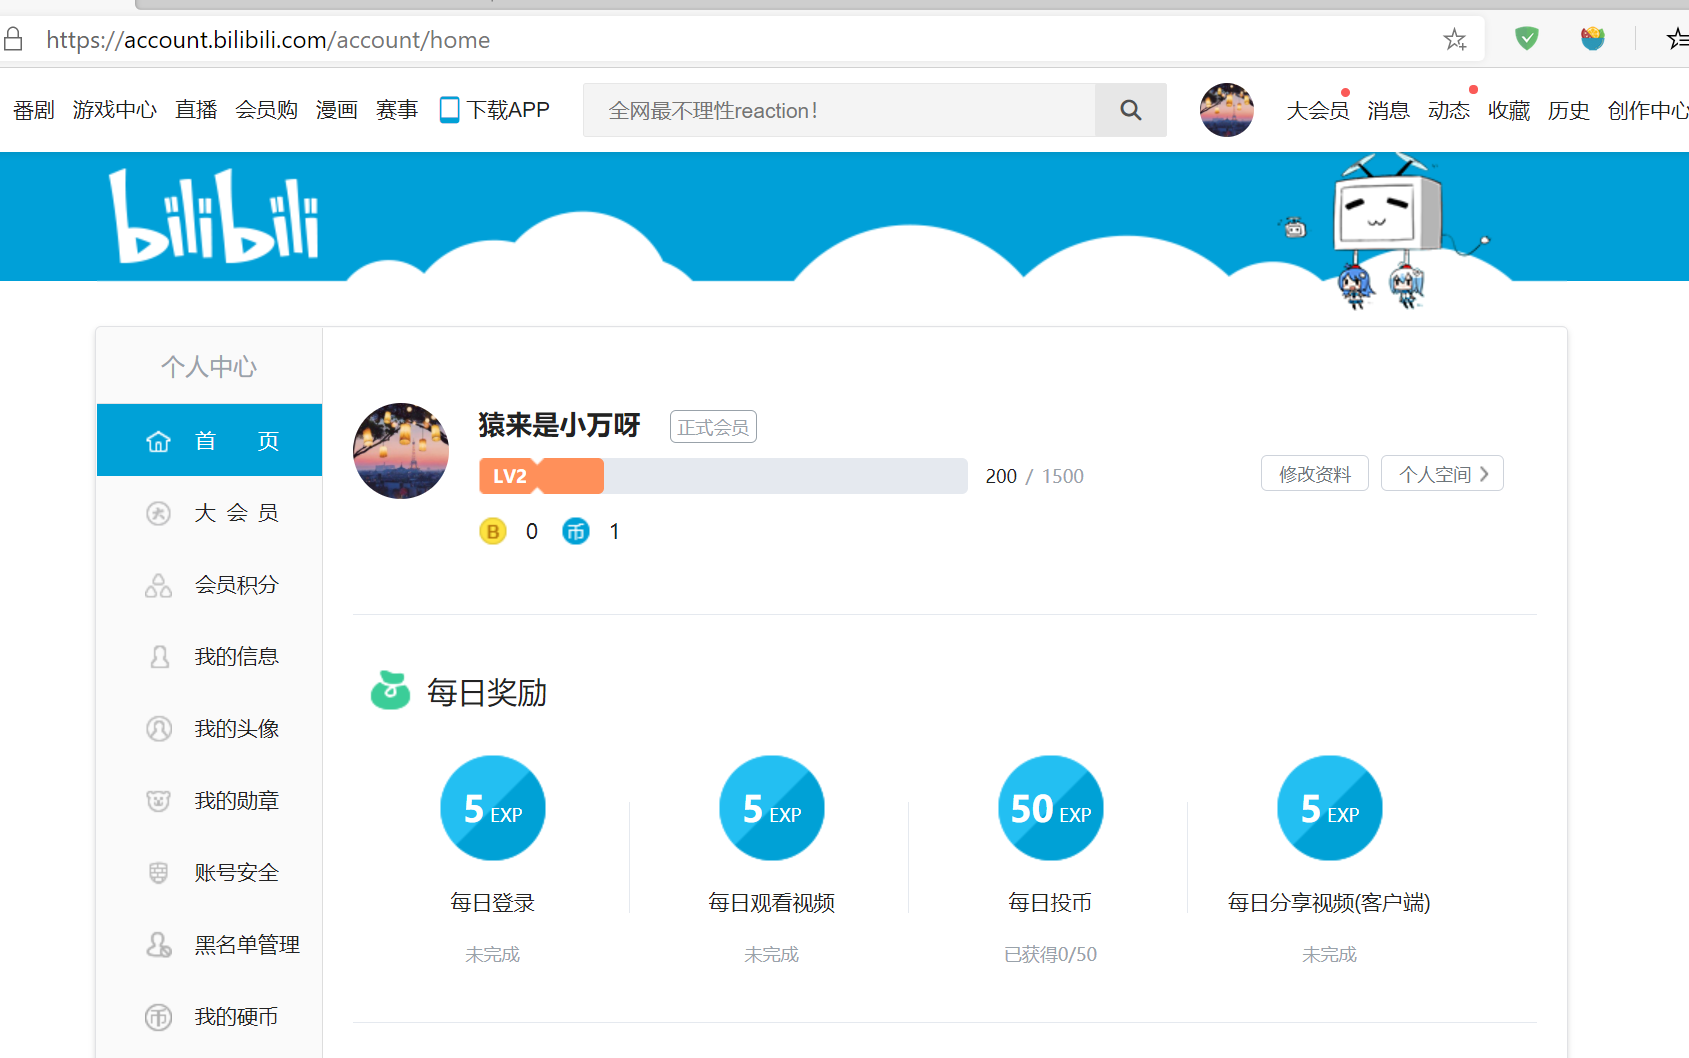
\includegraphics[width=0.7\linewidth]{B站}
    	\caption{}
    	\label{fig:b}
    \end{figure}
    
    \begin{figure}[H]
    	\centering
    	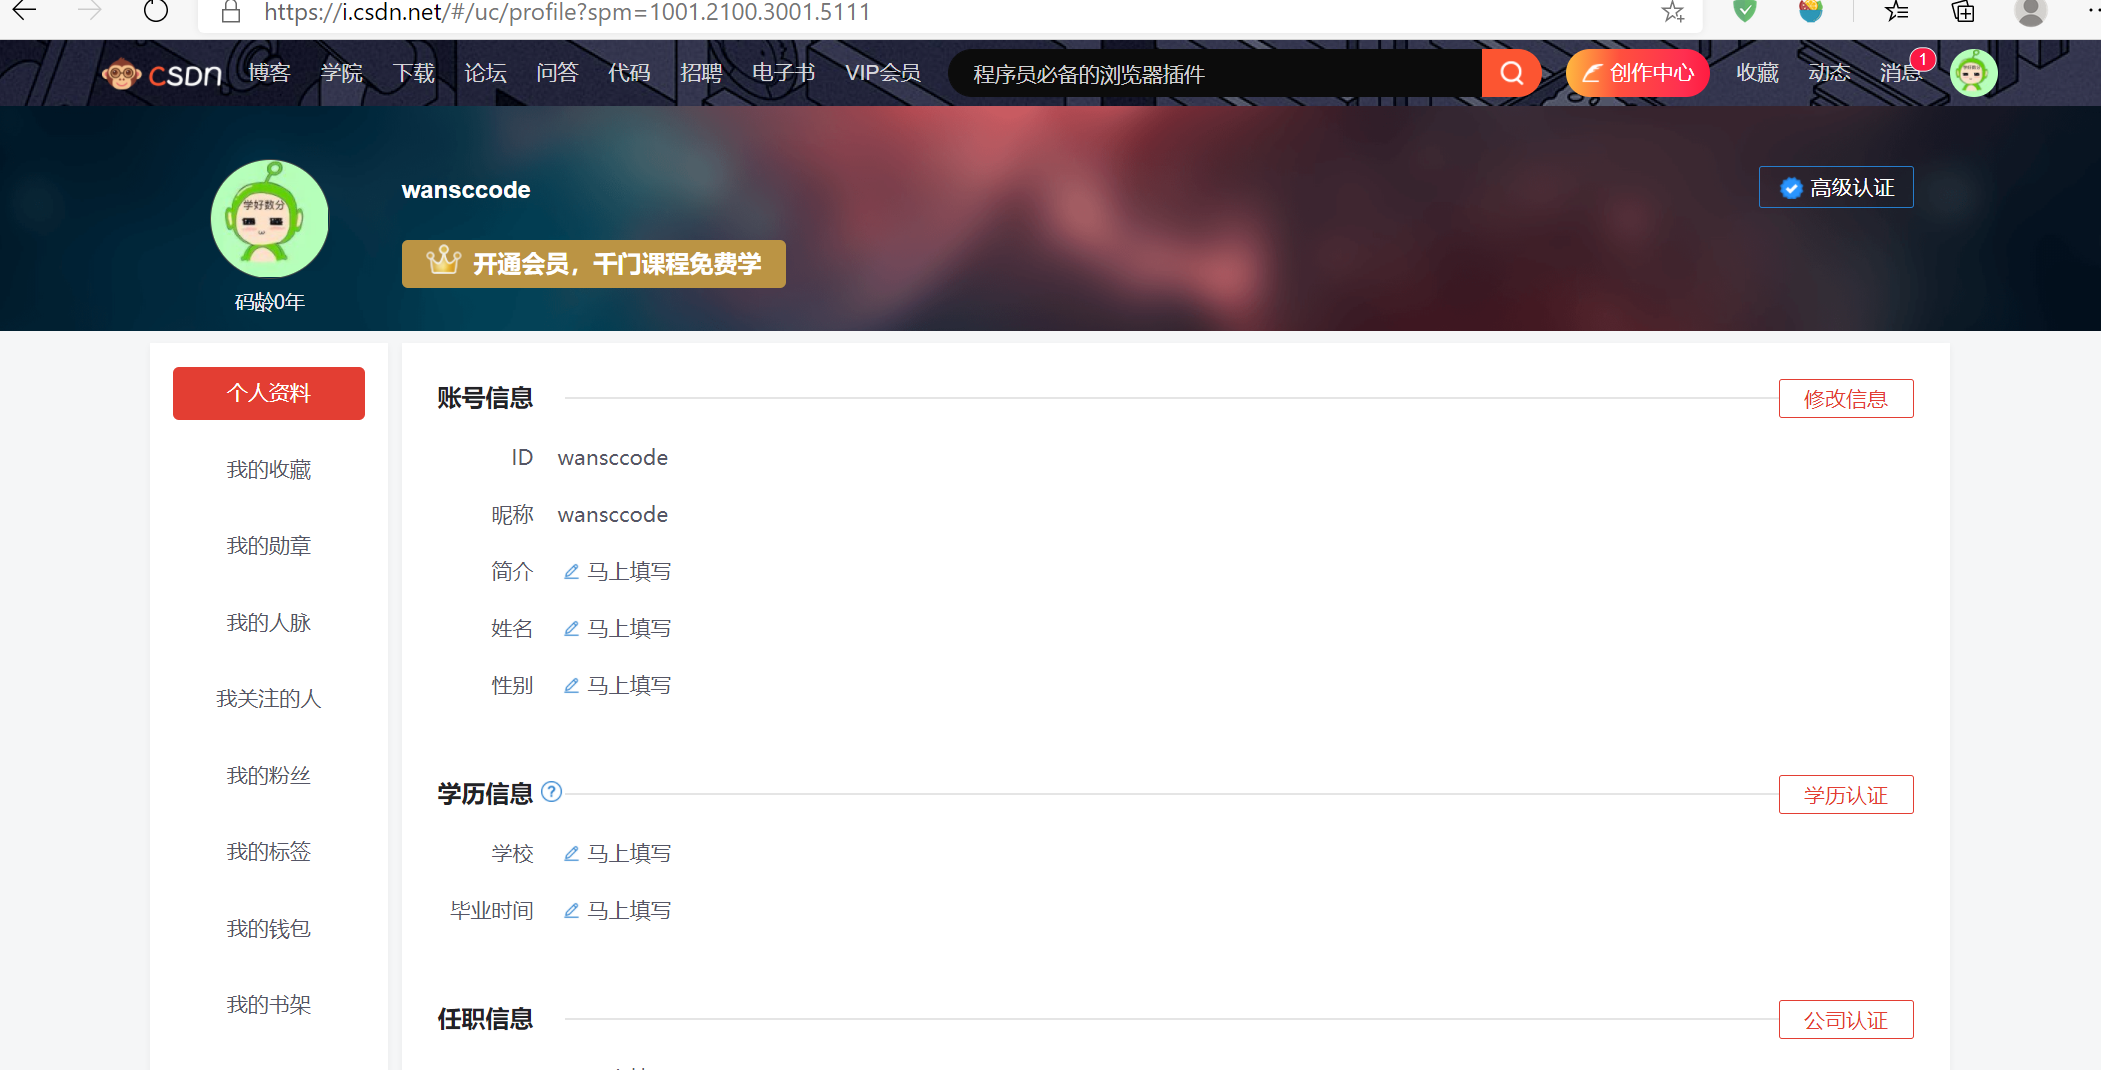
\includegraphics[width=0.7\linewidth]{CSDN}
    	\caption{}
    	\label{fig:csdn}
    	个人网址:https://blog.csdn.net/wansccode?spm=1010.2135.3001.5113
    \end{figure}
    
    
    \begin{figure}[H]
    	\centering
    	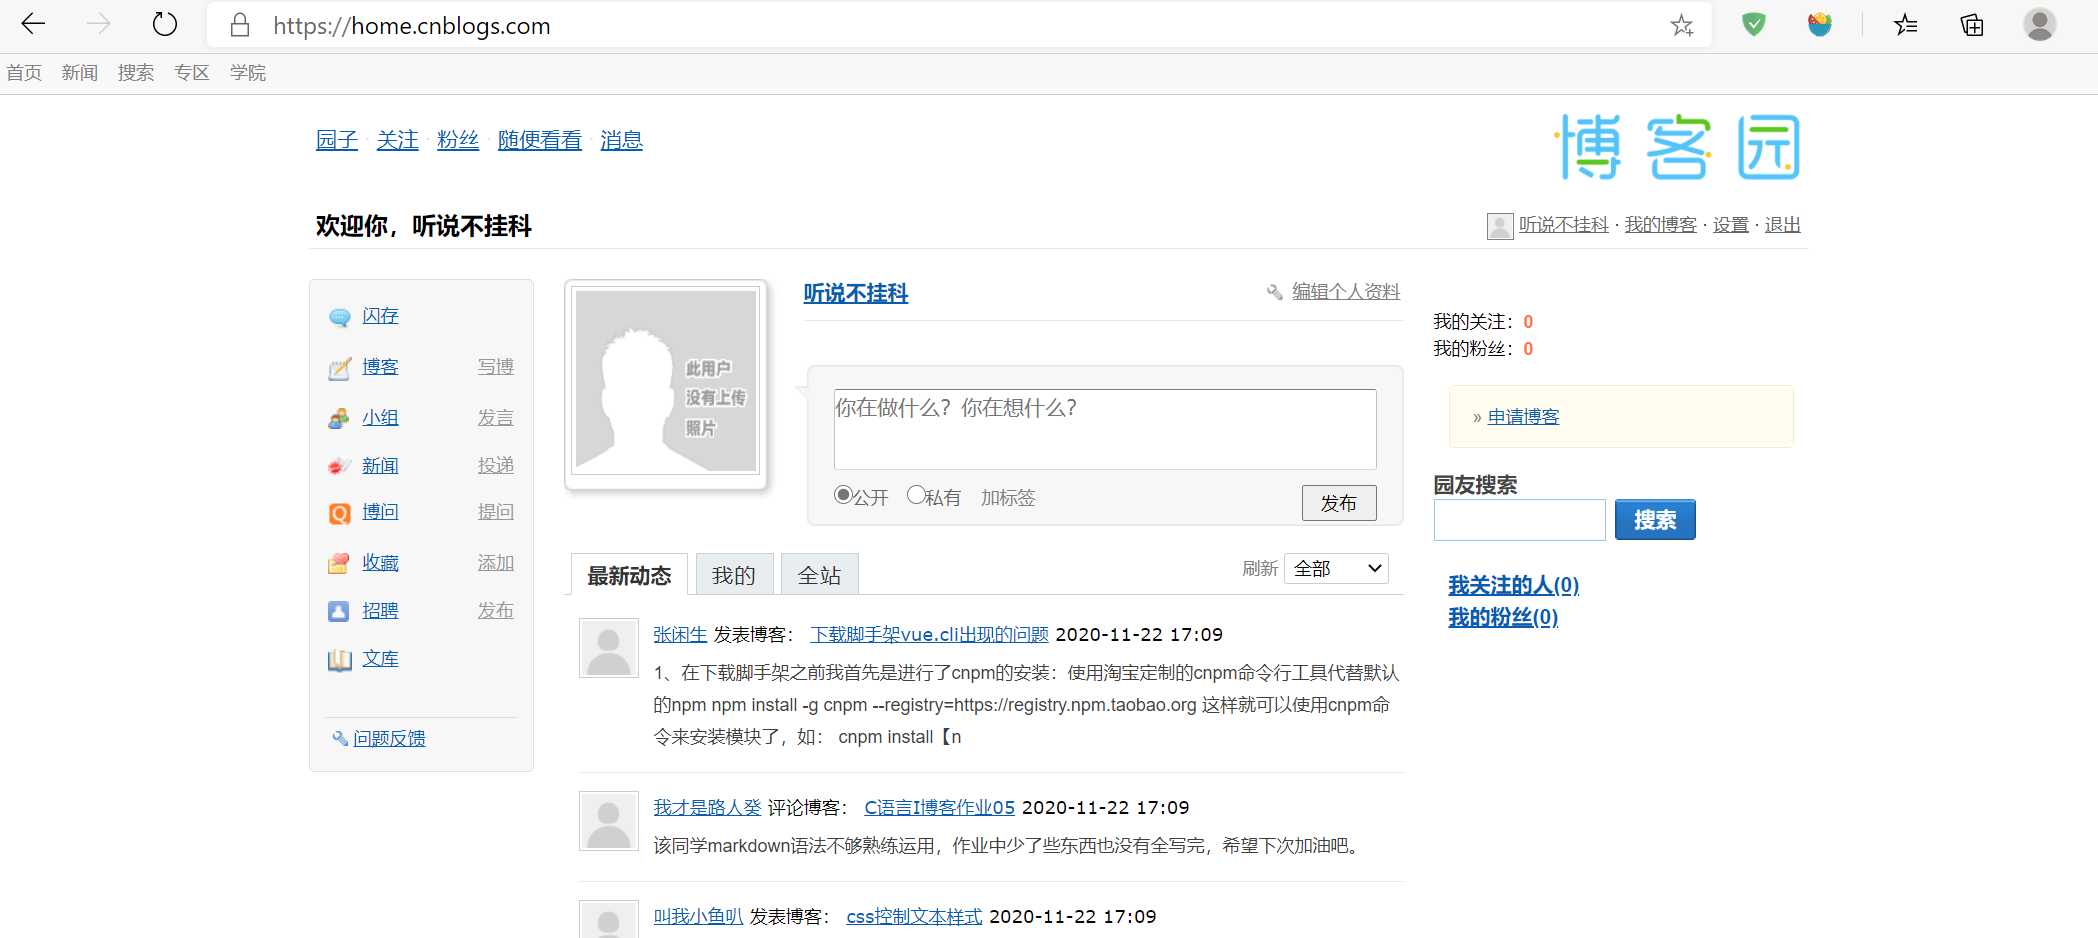
\includegraphics[width=0.7\linewidth]{博客园}
    	\caption{}
    	\label{fig:}
    	个人网址:https://home.cnblogs.com/
    \end{figure}
    
    
    \begin{figure}[H]
    	\centering
    	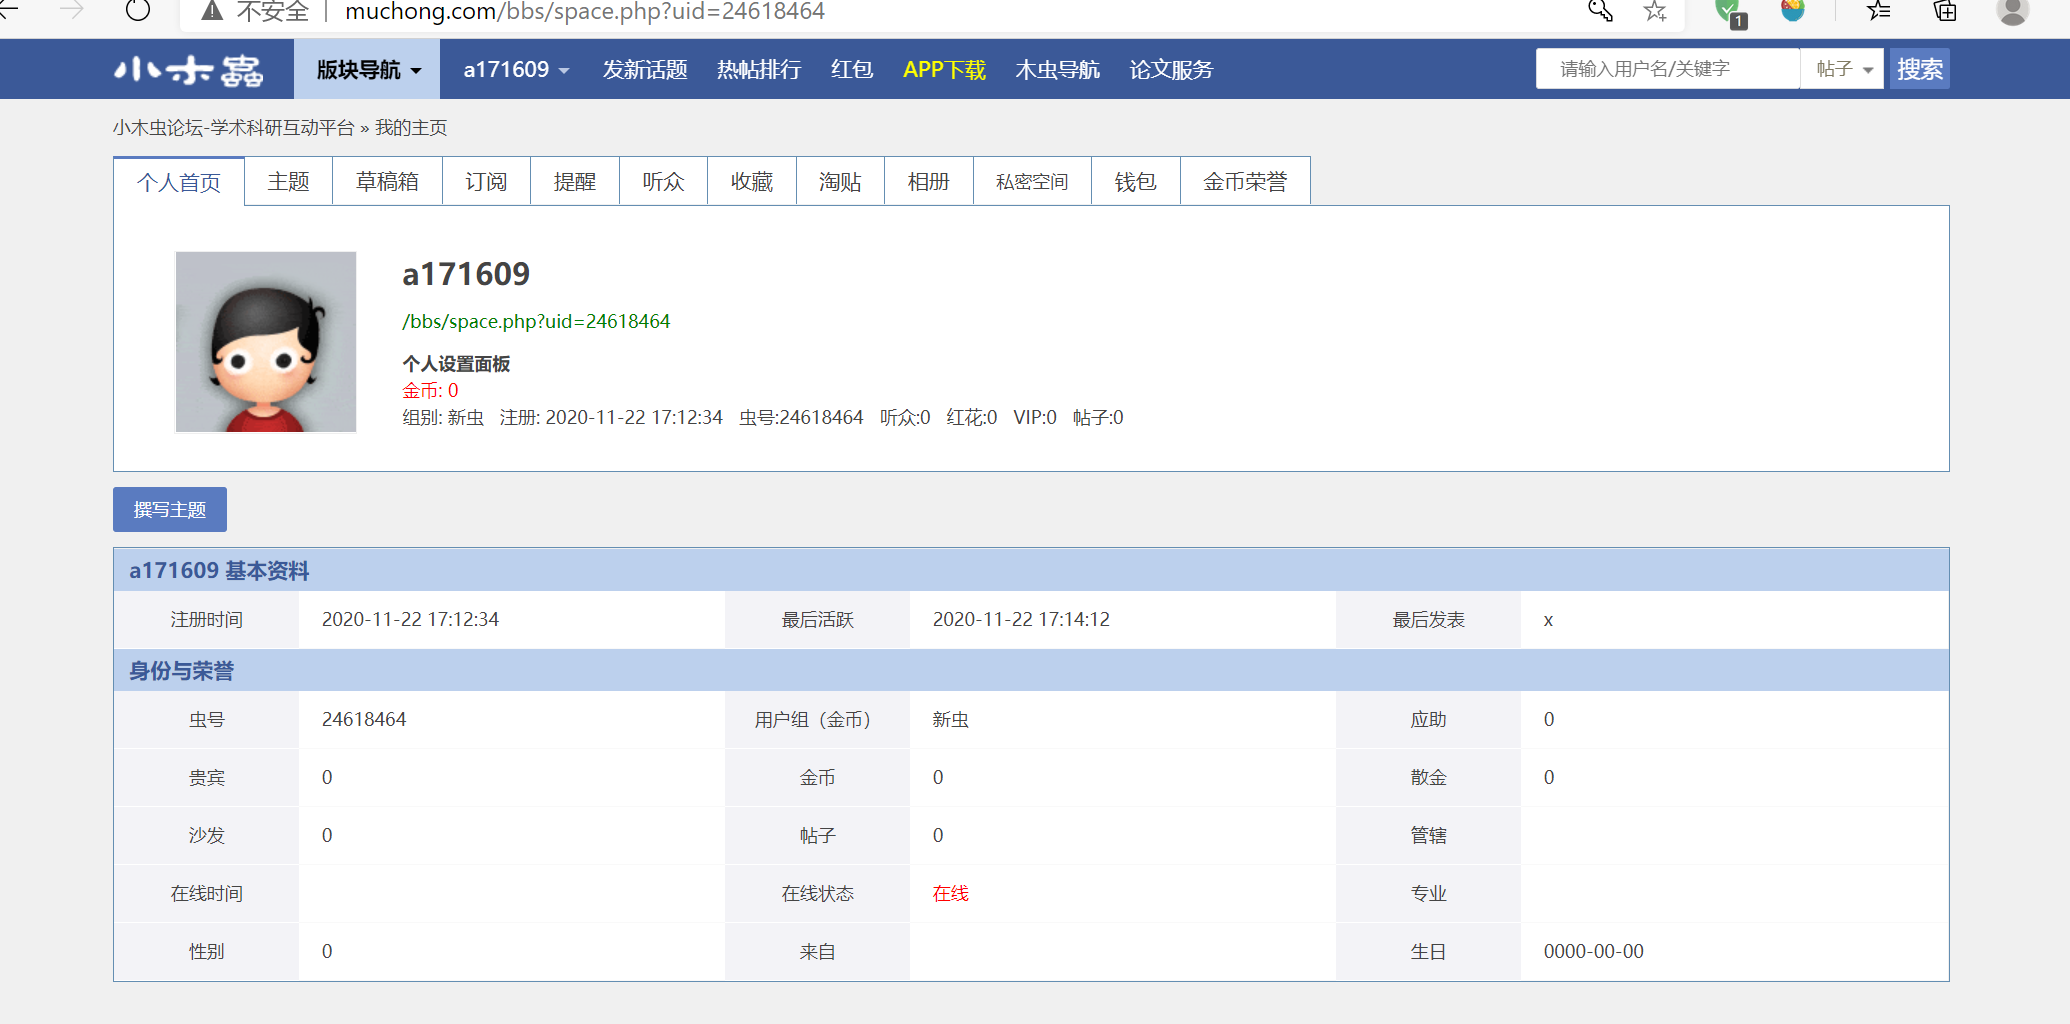
\includegraphics[width=0.7\linewidth]{小木虫}
    	\caption{}
    	\label{fig:}
    	个人网址:http://muchong.com/bbs/space.php?uid=24618464
    \end{figure}
    
    



\hspace*{\fill} \\

\bibliographystyle{unsrt}
\bibliography{references}


\end{document}
